%!TeX root = 5-diffusion.tex
\documentclass[main]{subfiles}

\begin{document}

\chapter{Xenon and krypton transport properties}
\vspace*{-1\baselineskip}

\section{Current state of the art}

Experiment? \todo{reprendre la review daglar}

\subsection{Molecular dynamics}

\subsection{Transition state theory}

\todo{what is a transition state for diffusion?}

\todo{how to detect TS}

Fast kinetic Monte Carlo
tutrast\autocite{Mace_2019}

\subection{ML modeling}

Results

\section{Transport properties of xenon/krypton separation}

\subsection{Why studying diffusion for xenon krypton}

\todo{kinetic KAXQIL problem}

\subsection{Correlations}

\section{Fast diffusion calculation algorithm}

\subsection{Implementation in C++}

\subsection{Preliminary results}

\subsection{Visualization tool}

\todo{Take some examples for the vizualisation with comparison to the pore size and diffusion coefficient}

\subsection{Development of a first prediction model}

\begin{figure}[ht]
  \centering
    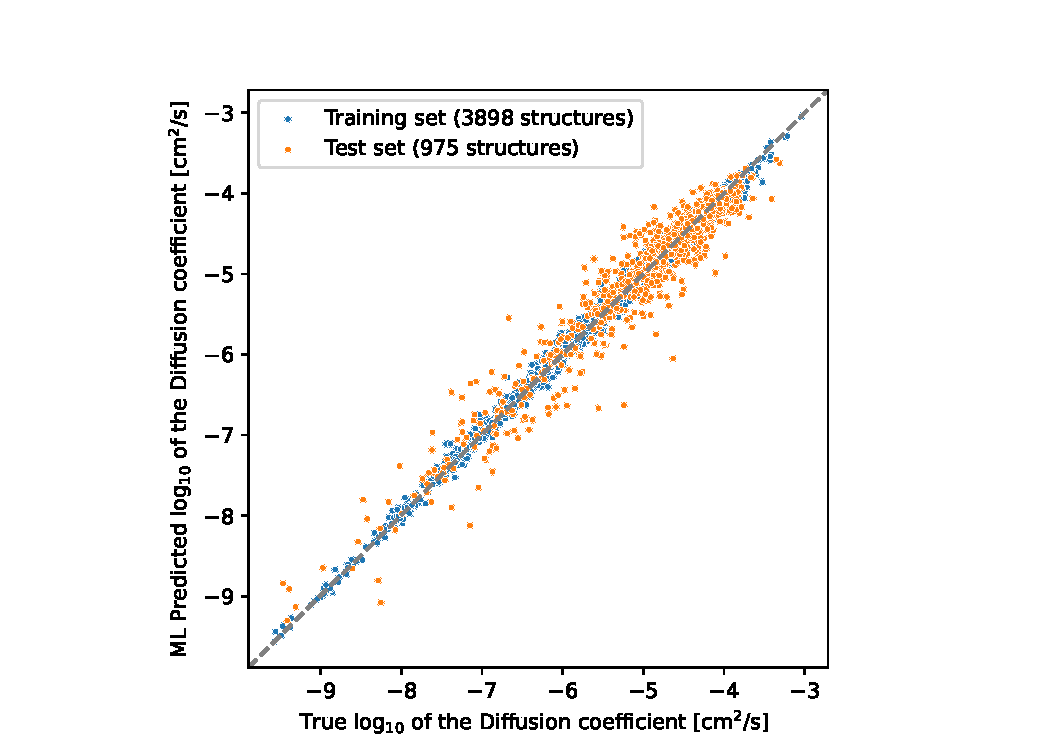
\includegraphics[width=6cm]{figures/5-diffusion/diffusion_prediction.pdf}
    \caption{}
    \label{fgr:}
\end{figure}

\begin{figure}[ht]
  \centering
    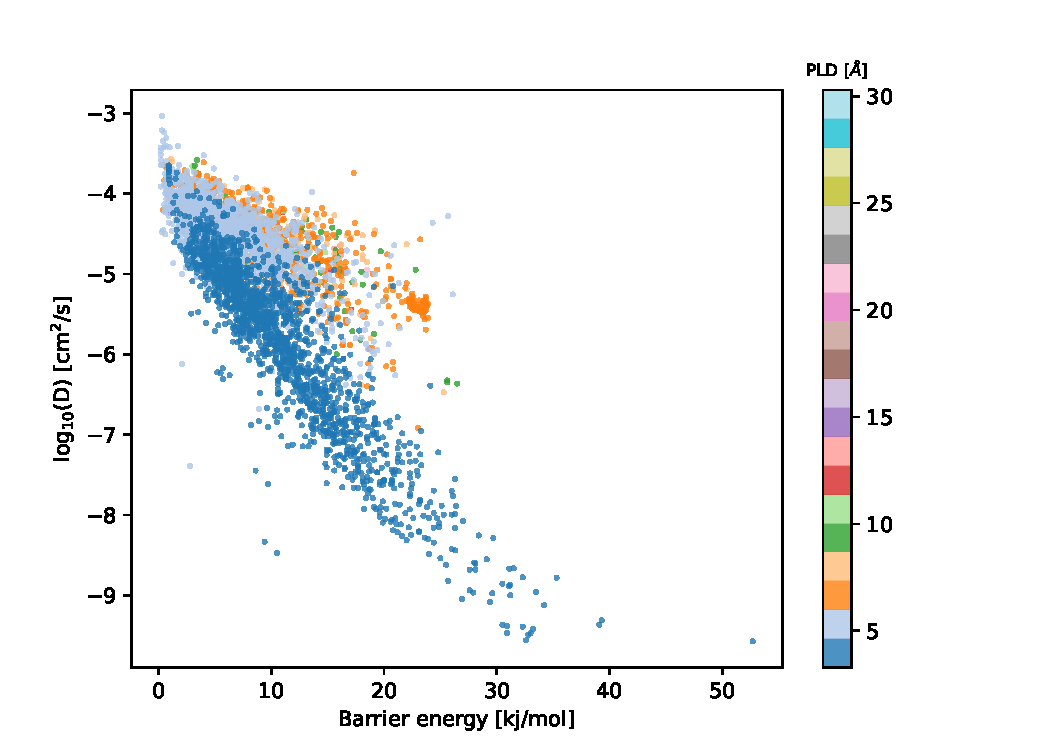
\includegraphics[width=0.48\textwidth]{figures/5-diffusion/difflog_barrier_Df_uff.pdf}
    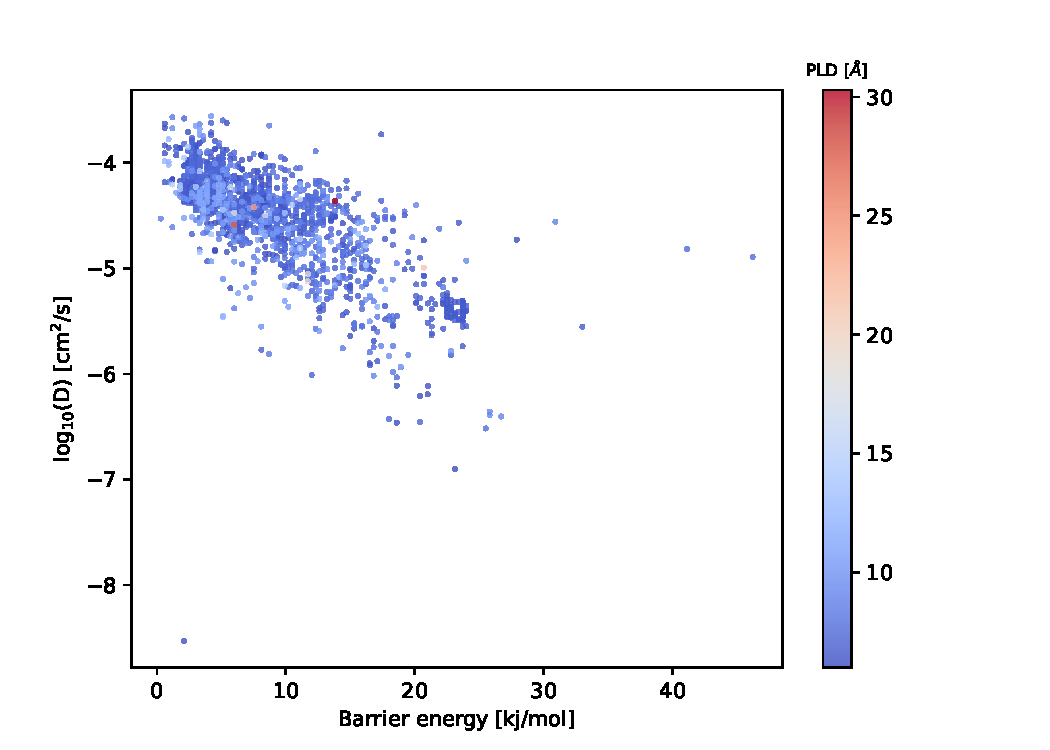
\includegraphics[width=0.48\textwidth]{figures/5-diffusion/difflog_barrier_Df_uff_2.pdf}
    \caption{}\label{fgr:}
\end{figure}

\begin{figure}[ht]
  \centering
    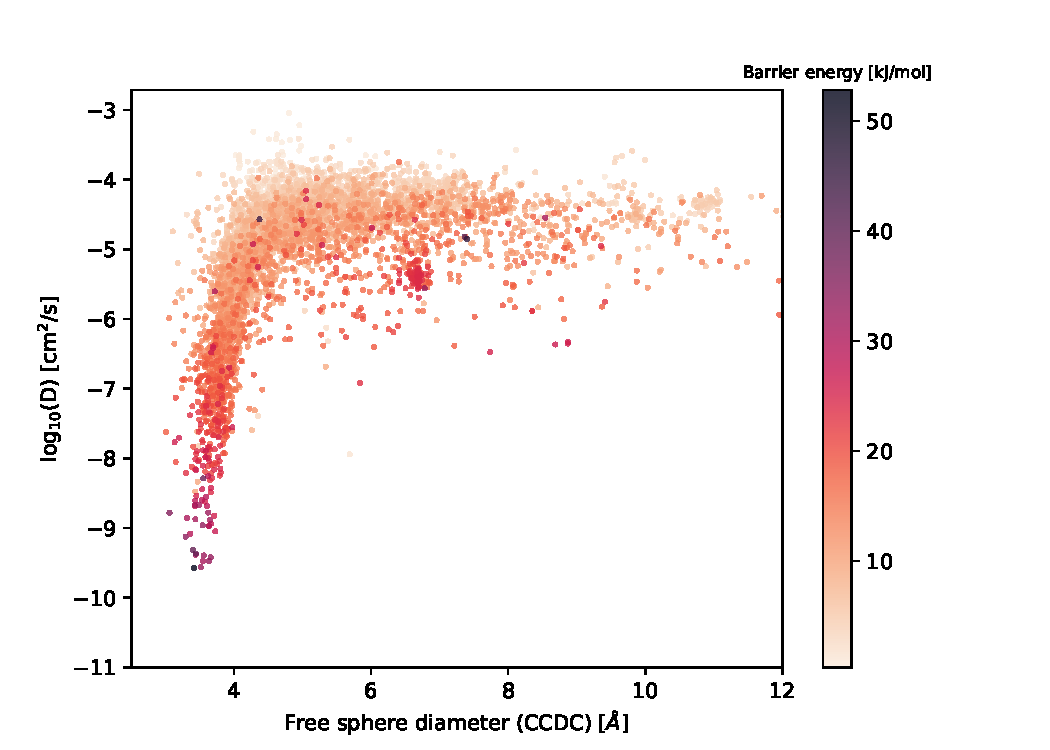
\includegraphics[width=0.48\textwidth]{figures/5-diffusion/difflog_Df-ccdc_barrier.pdf}
    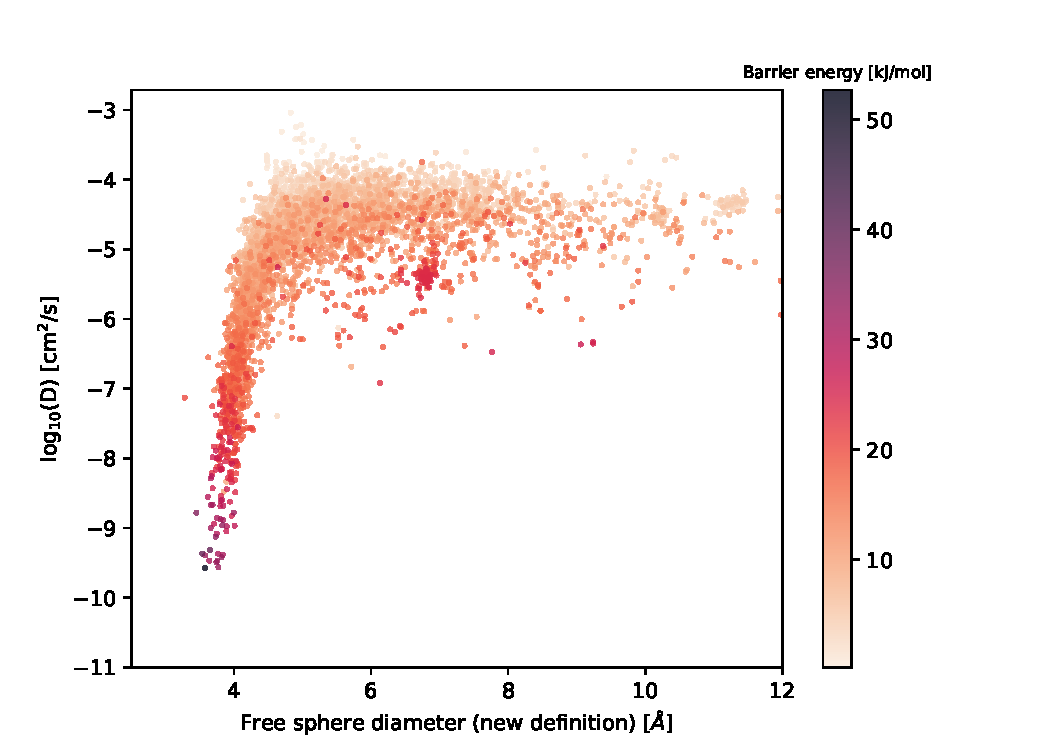
\includegraphics[width=0.48\textwidth]{figures/5-diffusion/difflog_Df-uff298K_barrier.pdf}
    \caption{}
    \label{fgr:}
\end{figure}

ML descriptors
next steps

\OnlyInSubfile{\printglobalbibliography}

\end{document}
